%%
% BIThesis 本科毕业设计论文模板 —— 使用 XeLaTeX 编译 The BIThesis Template for Undergraduate Thesis
% This file has no copyright assigned and is placed in the Public Domain.
%%

% 第一章节
\chapter{预备知识}

\section{实验预备知识}

\subsection{PE文件}

\textcolor{black}{PE文件是Windows操作系统下的可执行文件形式,包括EXE(可执行文件),DLL(动态链接库),SYS(系统文件)等类型。}

\textcolor{black}{PE文件中包含PE文件头(IMAGE\_NT\_HEADERS),其中的COFF文件头(IMAGE\_FILE\_HEADER)和可选首部(IMAGE\_OPTIONAL\_HEADER)中的有些部分是我们需要修改的目标。}]

\textcolor{black}{COFF文件头(IMAGE\_FILE\_HEADER)包含如下关键字段:}

\textcolor{black}{(1)Machine:目标CPU架构,指明了能运行这个程序的机器码,可以指明支持程序运行的机器架构是x86、x64、PowerPC、ARM等。}

\textcolor{black}{(2)NumberOfSections:指明所有节区的数量。}

\textcolor{black}{(3)TimeDateStamp:时间戳,指明了这个文件被编译生成的时间。}

\textcolor{black}{(4)SizeOfOptionalHeader:可选首部的大小。}

\textcolor{black}{(5)Characteristics:文件的类型,是动态链接库,还是可执行文件等类型。}

\textcolor{black}{可选首部(IMAGE\_OPTIONAL\_HEADER)包含如下字段,可选首部指明了当PE程序被载入内存后的一些情况:}

\textcolor{black}{(1)Magic:魔法位,包含PE信息,一定要和COFF文件头中的Machine对应,否则就会报错导致程序无法启动。}

\textcolor{black}{(2)AddressOfEntryPoint:程序入口点,即相对虚拟地址。}

\textcolor{black}{(3)ImageBase:加载机制。}

\textcolor{black}{(4)SectionAlignment:内存中节区的对齐粒度,不建议修改,否则程序可能无法启动。}

\textcolor{black}{(5)FileAlignment:文件中节区的对齐粒度,不建议修改,否则程序将无法启动。}

\textcolor{black}{(6)SizeOfImage:加载到内存后的总大小。}

\textcolor{black}{(7)SubSystem:子系统类型。}

\textcolor{black}{(8)DataDirectory:数据目录表,记录某些数据的位置及其大小。}

\textcolor{black}{PE文件中的节表(Section table)描述了每个节的属性,由多个IMAGE\_SECTION\_HEADER组成,每个条目对应一个节区,包括下列关键属性:}

\textcolor{black}{(1)Name:节区的名字。}

\textcolor{black}{(2)VirtualAddress:虚拟地址中的起始相对位置。}

\textcolor{black}{(3)SizeOfRawData:节区中数据的大小。}

\textcolor{black}{(4)PointerToRawData:节区偏移量。}

\textcolor{black}{(5)Characteristics:节区属性。}

\textcolor{black}{节区数据正常情况下应包含如下内容:}

\textcolor{black}{(1).text:代码节,存放该PE程序执行的指令。}

\textcolor{black}{(2).data:已经完成初始化的某些数据。}

\textcolor{black}{(3).rdata:只读(Read Only)的数据。}

\textcolor{black}{(4).rsrc:资源节,存放PE文件的图标等信息。}

\textcolor{black}{(5).reloc:重定位信息,可以用于动态链接库的装载过程。}

\textcolor{black}{(6).idata:import data,即导入函数信息。}

\textcolor{black}{数据目录表中包含的内容如下:}

\textcolor{black}{(1)Import Table:导入表,用于存放该PE文件依赖的动态链接库和调用的某些函数。}

\textcolor{black}{(2)Export Table:导出表,可以用于存放这个PE文件封装好的函数,多半运用于动态链接库封装函数供其余PE程序调用使用。}

\textcolor{black}{(3)Relocation Table:重定位表,修复地址偏移相关问题。}

\textcolor{black}{(4)TLS:线程存储表,与多线程程序有关,存储线程初始化数据。}

\textcolor{black}{(5)Debug Directory:存放该PE程序的调试信息。}

\subsection{强化学习}

\textcolor{black}{基本概念相关:}

\textcolor{black}{(1)智能体:在强化学习中决策,行动,学习。智能体是一个感知者,能感知并且理解当前的状态,智能体是一个决策者,能够知道在一个状态下应该采取什么行动,智能体是一个执行者,通过改变状态从而获取奖励。}

\textcolor{black}{(2)状态:描述了智能体与环境的相对状况。}

\textcolor{black}{(3)状态空间:所有状态的集合。}

\textcolor{black}{(4)动作:智能体在某一状态下能选择的操作。}

\textcolor{black}{(5)动作空间:所有动作的集合。}

\textcolor{black}{(6)状态转移:当执行一个动作时,智能体可能从一个状态转移到另一个状态的过程。}

\textcolor{black}{(7)策略:智能体在每一个状态下应该采取什么样的动作,允许分为确定性策略和随机性策略。}

\textcolor{black}{(8)奖励:作为人机交互的一个重要手段,可以设置合适的奖励来引导智能体按照我们的预期选择正确的决策,正数奖励表明我们鼓励智能体执行该行动,负数奖励表明我们不鼓励智能体执行该行动。}

\textcolor{black}{(9)回合/尝试:智能体执行一个策略与环境交互的过程中,智能体从开始状态到终止状态停止的过程被称为一个回合或尝试,一般用英文episode来表示。}

\textcolor{black}{(10)折扣因子:用于调整智能体对于近期奖励和远期奖励的重视程度,可以记作折扣因子为$\gamma$,$\gamma$在(0,1)的范围,且折扣因子的引入允许了无限长的轨迹。}

\textcolor{black}{(11)状态值:表达式如式(2-1)所示:}
\begin{equation}
v_{\pi}(s)=E[G_{t}|s_{t}=s]
\end{equation}

\textcolor{black}{状态值说明智能体在一个状态之下,最终能获取到的回报。首先,需要了解基于时序差分策略的方法可被用于估计状态值。}

\textcolor{black}{时序差分方法的表达式若式(2-2)所示:}
\begin{equation}
v_{t+1}(s_{t})  =v_{t}(s_{t})-\alpha_{t}(s_{t})[v_{t}(s_{t})-(r_{t+1}+\gamma v_{t}(s_{t+1}))],
v_{t+1}(s)=v_{t}(s)(s\neq s_{t})
\end{equation}

\textcolor{black}{$v_{t}(s_{t})$代表$t$时刻对于$v_{\pi}(s_{t})$的估计,${\alpha_{t}(s_{t})}$是$t$状态下对于状态$s_{t}$的学习率。}

\textcolor{black}{在$t$时刻,只有当时正在被访问的状态$s_{t}$的估计值会被更新。}

\textcolor{black}{在式(2-2)中:}

\textcolor{black}{$r_{t+1}+\gamma v_{t}(s_{t+1})$作为时序差分方法的目标。}

\textcolor{black}{$v_{t}(s_{t})-(r_{t+1}+\gamma v_{t}(s_{t+1}))$作为时序差分方法的误差。}

\textcolor{black}{$\alpha_{t}(s_{t},a_{t})$为在{t}时刻对于状态$s_{t}$的学习率}

\textcolor{black}{$v_{t+1}(s_{t})$为新的$t+1$时刻对于状态值$v_{\pi}(s)$的估计值。}

\textcolor{black}{$v_{t}(s_{t})$为$t$时刻对于状态$s\in\ S$的状态值$v_{\pi}(s)$的估计值。}

\textcolor{black}{Sarsa(state action reward action state action)是基于时序查分方法的强化学习算法,但是该方法不是估计状态值而是估计动作值\parencite{ref29},\parencite{ref30}。}

\textcolor{black}{首先要引入动作值的概念:}

\textcolor{black}{对于一个状态-动作配对${(s,a)}$,动作值定义表达式如式(2-3)所示。}
\begin{equation}
q_{\pi}\left({s,a}\right)={E}\left[\left.{G}_{t}\right|{S}_{t}{=s,} {A}_{t}{=a} \right] 
\end{equation}

\textcolor{black}{动作值表示在一个状态采取一个动作之后获得回报的期望值。}

\textcolor{black}{这里将${q}_{\pi}\left({s,a}\right)$的估计值记作${q}_{t}\left({s,a}\right)$。}

\textcolor{black}{给定一个策略$\pi$,需要估计其动作值,可以从$\pi$的经验样本中,使用Sarsa算法来估计动作值,其表达式为式(2-4),其中学习率为$\alpha _{t}(s_{t},a_{t})$。}
\begin{equation}
q_{t+1}(s_{t},a_{t})=q_{t}(s_{t},a_{t})-\alpha _{t}(s_{t},a_{t})[q_{t}(s_{t},a_{t})-(r_{t+1}+\gamma q_{t}(s_{t+1},a_{t+1}))]    
\end{equation}

\textcolor{black}{\ \ \ $q_{t+1}(s,a)=q_{t}(s,a) \ while \ (s,a) \neq (s_{t},a_{t})$}

\textcolor{black}{在t时刻,只有$\left({s}_{t}{,} {a}_{t}\right)$的动作值被更新,其它的动作值保持不变。}

\textcolor{black}{Sarsa算法主要是用于求解Bellman方程近似算法,近似算法的表达式如式(2-5)所示:}
\begin{equation}
{q}_{\pi}({s,a}){=E}[R+\gamma q_{\pi}(S',A')|_{(s,a)} \ for \ all \ (s,a) 
\end{equation}

\textcolor{black}{式(2-5)是一个基于动作值而不是状态值的Bellman方程。}

\textcolor{black}{图\ref{fig:sarsa}中的伪代码描述了如何运用Sarsa算法学习最优策略的执行逻辑。}

\begin{figure}
  \centering
  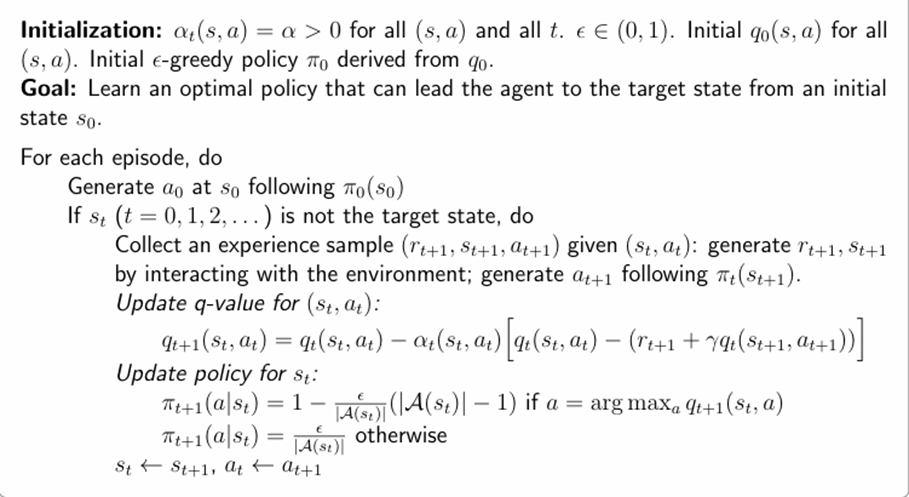
\includegraphics[]{images/sarsa.png}
  \caption{sarsa}\label{fig:sarsa}
\end{figure}

\textcolor{black}{目标:学习最优策略,使智能体能从给定状态$s_{0}$到达目标状态。}

\textcolor{black}{对于图2-1中的Sarsa算法描述如下所示:}

\textcolor{black}{算法初始化:}

\textcolor{black}{对于所有$\left({s,a}\right)$数值和所有$t$数值,选取学习率因子${\alpha}_{t}\left({s,a}\right) = {\alpha}$,贪婪因子${\epsilon}\in({0,1})$,并且设定所有$\left({s,a}\right)$的初始值为${q}_{0}\left({s,a}\right)$,从${q}_{0}$获取初始贪婪策略${\pi}_{0}$。}

\textcolor{black}{算法目标:学习最优策略,使智能体能从给定的状态${s}_{0}$出发,到达目标终止状态。}

\textcolor{black}{对于每个回合:}

\textcolor{black}{\ \ 如果当前状态是${s}_{0}$根据$ {\pi}_{0}\left({s}_{0}\right)$,选取策略 $a ={a}_{0}$}

\textcolor{black}{\ \  在时刻t,如果${s}_{t}$不是目标状态}

\textcolor{black}{\ \ \ \  收集经验样本$({s}_{t}, {a}_{t}, {s}_{{t+1}}, {a}_{{t+1}})$:在${s}_{t}$通过与环境交互生成${r}_{{t+1}},{s}_{{t+1}}$。}

\textcolor{black}{\ \ \ \ 再根据${\pi}_{t}\left({s}_{{t+1}}\right)$生成 ${a}_{{t+1}}$}

\textcolor{black}{\ \ \ \  随后更新$({s}_{t}, {a}_{t})$的值}

\textcolor{black}{Sarsa算法也存在一些推广,例如Expected Sarsa算法、n-step Sarsa算法等,尽管本实验中并未涉及到这些推广算法,但是读者在构建强化学习对抗性样本生成模型上也可以尝试使用它们。}

\textcolor{black}{其中Expected Sarsa算法类似Sarsa算法,但是它们的时序差分方法目标上不同。具体实现流程上二者相似。}

\textcolor{black}{已知策略$\pi$,则Expected Sarsa算法对于该策略$\pi$的动作值估计公式如式(2-6)所示:}
\begin{equation}
q_{t+1}(s_{t},a_{t})=q_{t}(s_{t},a_{t})-\alpha _{t}(s_{t},a_{t})[q_{t}(s_{t},a_{t})-(r_{t+1}+\gamma E[q_{t}(s_{t+1},a_{t+1})])] 
\end{equation}

\textcolor{black}{\ $q_{t+1}(s,a)=q_{t}(s,a) \ while \ (s,a) \neq (s_{t},a_{t})$}

\textcolor{black}{在式(2-6)中:}
\begin{equation}
    E[q_{t}(s_{t+1},a)]=\Sigma_{a}\pi_{t}(a|s_{t+1})q_{t}(s_{t+1},a)=v_{t}(s_{t+1})
\end{equation}

\textcolor{black}{式(2-7)是在策略${\pi}_{t}$下${q}_{t}\left({s}_{{t+1}}{,a} \right)$的期望值。}

\textcolor{black}{不同于Sarsa算法的目标是求出$r_{t+1}+\gamma q_{t}(s_{t+1},a_{t+1})$,Expected Sarsa算法的目标是求出$r_{t+1}+\gamma E[q_{t}(s_{t+1},a_{t+1})]$。}

\textcolor{black}{引入期望值会增加计算复杂度,但是会减小所求目标的方差,Expected Sarsa的涉及的随机变量是${{s}_{t}{,}a_t,r_{t+1},s_{t+1}}$,相比Sarsa算法的${s_t,a_t,r_{t+1},s_{t+1},a_{t+1}}$,减少了一项,因此对于减少估计方差是有正面作用的\parencite{ref30},\parencite{ref31},\parencite{ref32}。}

\subsection{恶意软件种类}

\textcolor{black}{(1)病毒}

\textcolor{black}{计算机病毒是具有自我复制性的一段计算机命令或代码段,可以将自身插入到其他程序中,进而感染其他程序实行自我复制,这可能会造成用户的数据丢失以及计算机系统功能受损,被病毒感染的文件可以通过U盘,移动光盘等外部设备进行传播。计算机病毒大多数需要依附于受感染的程序被用户运行来传播,同时,计算机病毒具有高隐蔽性。}

\textcolor{black}{(2)木马}

\textcolor{black}{特洛伊木马是伪装成恶意程序的正常应用程序,实际上特洛伊木马被黑客植入了恶意功能。木马能够允许远程黑客对计算机实现入侵,窃取本机的重要数据和信息,同时,木马创立的远程连接也能够供黑客组建僵尸网络,发动DDOS攻击等行为。不同于病毒,特洛伊木马不会复制自身,但目前存在木马下载器变种,当木马下载器被运行时,可能会下载其他的病毒和木马程序到受感染的机器。}

\textcolor{black}{(3)后门程序}

\textcolor{black}{后门程序允许黑客绕过安全监测对计算机进行攻击,具有高隐蔽性。它的来源有多种。一部分是因为软件开发人员的失误问题,在软件的开发工程中,可能开发人员为了软件便于测试,会主动设计一些后门,例如测试使用的超级用户,然而,在正式版软件被发布前,这些预设的后门理论上应该被开发人员主动删除以避免软件存在的安全问题,但很可能软件开发人员会有遗漏,而这些被遗漏的后门很有可能被黑客利用向计算机发动攻击。另一部分后门是黑客在对某机器成功实现攻击后,为了以后能利用这台主机作为跳板对其他机器实施新的攻击,黑客会在被攻击的机器上主动安装后门程序。}

\section{本章小结}

\textcolor{black}{本章对论文研究的相关技术理论予以介绍,首先介绍了实验的目标-PE可执行文件的结构,之后介绍了强化学习的基本知识和基于时序查分方法的Sarsa算法,最后介绍了恶意软件的种类知识,包括病毒,特洛伊木马,后门程序等。}